%----------------------------------------------------------------------------------------
%    PACKAGES AND THEMES
%----------------------------------------------------------------------------------------

\documentclass[handout,aspectratio=169,xcolor=dvipsnames,10pt]{beamer}
\usetheme{SimplePlus}

\usepackage{hyperref}
\usepackage{graphicx} % Allows including images
\usepackage{booktabs} % Allows the use of \toprule, \midrule and \bottomrule in
\usepackage{xcolor}
\definecolor{lightblue}{rgb}{0.68, 0.85, 0.9}
\definecolor{junglegreen}{rgb}{0.16, 0.67, 0.53}
\definecolor{dodgerblue}{rgb}{0.12, 0.56, 1.0}
\definecolor{nicered}{rgb}{0.9, 0.17, 0.31}
\definecolor{darkblue}{rgb}{0.0, 0.48, 0.65}

\usepackage{tikz}
\usetikzlibrary{arrows.meta,positioning,shapes.geometric,shapes,arrows,fit,calc,backgrounds,decorations.pathreplacing}

% Unified TikZ styles
\tikzset{
  >={Stealth[length=5pt]},
  object/.style={circle,draw,thick,fill=lightblue,minimum size=10mm,font=\small},
  machine/.style={rectangle,draw,thick,rounded corners=4pt,minimum width=4.2cm,minimum height=3cm,fill=gray!5,dashed},
  controller/.style={rectangle,draw,thick,rounded corners=2pt,minimum width=3.8cm,minimum height=2.4cm,fill=gray!10},
  edge/.style={->,thick,draw=darkblue},
  msg/.style={edge,draw=dodgerblue},
  resp/.style={edge,draw=junglegreen},
  state/.style={rectangle,draw,thick,rounded corners=2pt,minimum width=2.6cm,minimum height=1cm},
  final/.style={state,fill=junglegreen!30,minimum width=2.4cm,minimum height=0.9cm},
  abort/.style={state,fill=nicered!25,minimum width=2.4cm,minimum height=0.9cm},
  event/.style={rectangle,fill=junglegreen!60,draw,thick,rounded corners=2pt,minimum width=2cm,minimum height=0.8cm},
  result/.style={rectangle,fill=dodgerblue!60,draw,thick,rounded corners=2pt,minimum width=1.2cm,minimum height=0.8cm},
  silent/.style={circle,fill=gray!30,draw,thick,minimum size=6mm},
  brace/.style={decorate,decoration={brace,amplitude=8pt}}
}
\usepackage{eso-pic}
\usepackage{transparent}

% Bibliography
\usepackage[numbers,sort&compress]{natbib}
\bibliographystyle{alpha}

% Font configuration for code (with fallback)
\usepackage{fontspec}
% these lines cause trouble
% \IfFontExistsTF{PragmataPro Mono}{%
%   \setmonofont{PragmataPro Mono}[Scale=1.0,Contextuals=Alternate]%
% }{%
%   \setmonofont{Inconsolata}[Scale=0.95]%
% }
% thus we take the following three instead
\usepackage{newunicodechar}
\newunicodechar{ℕ}{\ensuremath{\mathbb{N}}}
\newunicodechar{⊤}{\ensuremath{\top}}


% Code listings for Agda
\usepackage{listings}
% Light theme code highlighting for listings
\definecolor{codebg}{RGB}{248,249,250}
\definecolor{codeframe}{gray}{0.85}
\definecolor{codekw}{rgb}{0.00,0.28,0.45}   % dark blue
\definecolor{codecm}{rgb}{0.38,0.38,0.38}   % mid gray
\definecolor{codestr}{rgb}{0.55,0.00,0.08}  % deep red
\definecolor{codeid}{rgb}{0.00,0.65,0.31}   % bright green (for emph)

\lstdefinestyle{lightcode}{
  language=Haskell,
  basicstyle=\ttfamily\small,
  columns=flexible,
  breaklines=true,
  mathescape=true,
  escapeinside={(*}{*)},
  showstringspaces=false,
  backgroundcolor=\color{codebg},
  frame=single,
  rulecolor=\color{codeframe},
  frameround=fftt,
  framesep=3pt,
  xleftmargin=0.5em,
  xrightmargin=0.5em,
  keywordstyle=\color{codekw}\bfseries,
  commentstyle=\color{codecm}\itshape,
  stringstyle=\color{codestr},
  % Enrich Haskell with Agda-ish constructs
  morekeywords={record,field,Set,module,open,import,with,let,in,do,if,then,else,case,of,return,data,where},
  % Emphasize ISA operations
  emph={beginTx,commitTx,abortTx,call,self,input,scry,reflect,teleport,transferObject,createObj,destroyObj,receive,sender,history,getCurrentMachine,getMachine,moveObject,fetch,freeze,getCurrentController,getController,newVar,narrow,post,label,choose,require,reifyContext,reifyTxState,reifyConstraints,scryMeta,scryDeep,callPure,registerPure,updatePure,newLinearConstraint,satisfyLinear},
  emphstyle=\color{codeid}\bfseries,
  literate={→}{$\to$}1 {∀}{$\forall$}1 {λ}{$\lambda$}1 {≡}{$\equiv$}1 {⊤}{$\top$}1 {⊕}{$\oplus$}1
}

\lstset{style=lightcode}

% For checkmarks and symbols in tables
\usepackage{amssymb}
\usepackage{pifont}
\newcommand{\cmark}{\ding{51}}
\newcommand{\xmark}{\ding{55}}

%----------------------------------------------------------------------------------------
%    TITLE PAGE
%----------------------------------------------------------------------------------------

\title{AVM: Anoma Virtual Machine}
\subtitle{Layered Instruction Set Architecture for Distributed Objects}
\author{\textbf{Jonathan Prieto-Cubides}, Tobias Heindel, Chris Goes, ...}
\institute{Anoma Research — Heliax AG}
\date{\today}
   % Date, can be changed to a custom date

%----------------------------------------------------------------------------------------
%    PRESENTATION SLIDES
%----------------------------------------------------------------------------------------

% (Per-section outline disabled for a cleaner flow)

\begin{document}

\begin{frame}
  \titlepage
\end{frame}

%------------------------------------------------

\begin{frame}{Talk Overview}

\vfill

\begin{enumerate}
  \item \textbf{The Challenge:} What makes distributed transactional objects hard?

  \vspace{0.5em}

  \item \textbf{The Design:} How do we organize the complexity?
  \begin{itemize}\small
    \item Where vs. Who: Physical and logical distribution
    \item Layered instruction set architecture
  \end{itemize}

  \vspace{0.5em}

  \item \textbf{The Details:} What can the AVM do?
  \begin{itemize}\small
    \item Objects, transactions, distribution
    \item Constraint programming for intent matching
  \end{itemize}

  \vspace{0.5em}

  \item \textbf{The Practice:} How does it work?
  \begin{itemize}\small
    \item Running example: Atomic transfer
  \end{itemize}

\end{enumerate}

\vfill

\end{frame}

%----------------------------------------------------------------------------------------
%    PART I: MOTIVATION & CONTEXT
%----------------------------------------------------------------------------------------

\section{Motivation \& Context}

%------------------------------------------------

\begin{frame}{What makes distributed transactional objects hard?}

\vfill

\textbf{Goal:} Machine-checked formal semantics for distributed transactional objects supporting intent-based composition

\vspace{0.8em}

\textbf{Key design challenges:}

\begin{enumerate}
  \item \textcolor{nicered}{Distribution vs. Atomicity} \\
  {\small Objects across controllers—how to compose multi-party transactions?}

  \item \textcolor{nicered}{Safety vs. Expressiveness} \\
  {\small Support reflection and introspection while maintaining encapsulation}

  \item \textcolor{nicered}{Execution vs. Matching} \\
  {\small Two constraint models: call-time choice (FD) vs. commit-time validation (intents)}

  \item \textcolor{nicered}{Semantics vs. Implementation} \\
  {\small Denotational specification independent of platform concerns (scheduling, persistence, etc.)}
\end{enumerate}

\vspace{0.5em}

{\small\textbf{Our approach:} Layered ISA + interaction trees + object-centric histories}

\vfill

\end{frame}

%------------------------------------------------

\begin{frame}{How have others approached this problem?}

\vfill

Software systems with overlapping goals:
\begin{itemize}
  \item \textbf{Distributed Erlang VM / BEAM (active):} Actor model, message-passing concurrency,
  fault-tolerance, built-in distribution; no transactional semantics.
  \item \textbf{Mozart/OZ VM (inactive):} Multi-paradigm language with lightweight concurrency,
  constraints, and transparent distribution.
  \item \textbf{GemStone/Smalltalk (active):} Distributed object-oriented database with
  multi-user transactional support.
  \item \textbf{Seamless/Pharo (active):} Distributed object middleware with transparent remote communication.
\end{itemize}

\vspace{0.5em}

Theoretical models with similar abstractions:
\begin{itemize}
  \item \textbf{Obliq (Cardelli) (inactive):} Distributed object language with lexically-scoped
  network objects and object migration primitives.
  \item \textbf{Transactional Object Calculus (Vitek \& Jagannathan) (inactive):} Formal calculus
  combining object-oriented features with transactional semantics.
  \item \textbf{Distributed Oz (Van Roy \& Haridi) (inactive):} Network-transparent distributed
  computation with mobile objects and constraint programming.
\end{itemize}

\vfill

\end{frame}

%------------------------------------------------

\begin{frame}{What is the AVM?}

\begin{columns}[T]
\column{0.52\textwidth}

The \textbf{Anoma Virtual Machine} is:

\begin{itemize}
  \item \textbf{Message-driven objects}
  \begin{itemize}\small
    \item Not functions, not actors
    \item Process message sequences
  \end{itemize}

  \vspace{0.3em}

  \item \textbf{Transactional semantics}
  \begin{itemize}\small
    \item Serializable snapshot isolation
    \item Single-controller atomic blocks
  \end{itemize}

  \vspace{0.3em}

  \item \textbf{Two-level distribution}
  \begin{itemize}\small
    \item \textbf{Machines:} Physical compute nodes
    \item \textbf{Controllers:} Logical authority domains
    \item Objects migrate between both
  \end{itemize}
\end{itemize}

\column{0.48\textwidth}
\centering

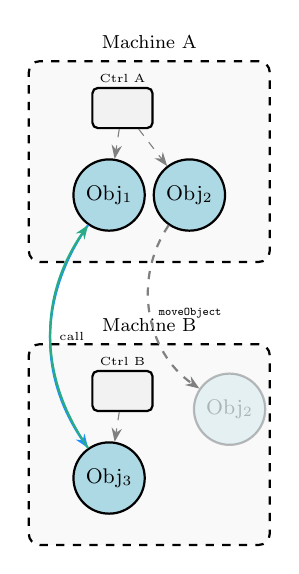
\begin{tikzpicture}[node distance=1cm,font=\small,scale=0.85,transform shape]
  % Machine A
  \node[machine,minimum width=3.6cm,minimum height=3cm] (ma) {};
  \node[above=0.05cm of ma,font=\footnotesize] {Machine A};

  % Machine B
  \node[machine,minimum width=3.6cm,minimum height=3cm,below=1.2cm of ma] (mb) {};
  \node[above=0.05cm of mb,font=\footnotesize] {Machine B};

  % Controllers (small boxes representing controller objects)
  \node[controller,minimum width=0.9cm,minimum height=0.6cm] (ca) at ([yshift=0.8cm,xshift=-0.4cm]ma.center) {};
  \node[above=-0.05cm of ca,font=\tiny] {Ctrl A};
  \node[controller,minimum width=0.9cm,minimum height=0.6cm] (cb) at ([yshift=0.8cm,xshift=-0.4cm]mb.center) {};
  \node[above=-0.05cm of cb,font=\tiny] {Ctrl B};

  % Objects (outside controllers, inside machines)
  \node[object,minimum size=6mm] (oa1) at ([yshift=-0.5cm,xshift=-0.6cm]ma.center) {Obj$_1$};
  \node[object,minimum size=6mm] (oa2) at ([yshift=-0.5cm,xshift=0.6cm]ma.center) {Obj$_2$};
  \node[object,minimum size=6mm] (ob1) at ([yshift=-0.5cm,xshift=-0.6cm]mb.center) {Obj$_3$};

  % Controller references to objects (dashed lines)
  \draw[edge,dashed,gray,thin] (ca) -- (oa1);
  \draw[edge,dashed,gray,thin] (ca) -- (oa2);
  \draw[edge,dashed,gray,thin] (cb) -- (ob1);

  % Message across controllers
  \draw[msg] (oa1) to[bend right=35] node[right,font=\tiny]{call} (ob1);
  \draw[resp] (ob1) to[bend left=35] (oa1);

  % Physical move (moveObject)
  \node[object,opacity=0.25,minimum size=6mm] (oa2ghost) at ([xshift=0.6cm,yshift=-3.2cm]oa2) {Obj$_2$};
  \draw[edge,dashed,gray] (oa2) to[bend right=45] node[right,font=\tiny,black]{\texttt{moveObject}} (oa2ghost);
\end{tikzpicture}

\end{columns}

\end{frame}

%------------------------------------------------

\begin{frame}{How is the specification structured?}

\vfill

\begin{center}
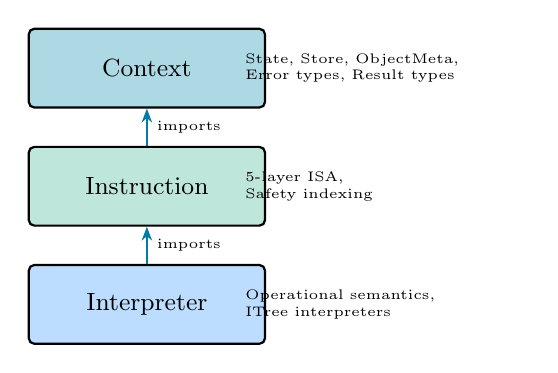
\begin{tikzpicture}[node distance=1.5cm,font=\small]
  % Three main modules
  \node[state,fill=lightblue,minimum width=3cm,minimum height=1cm] (context) {Context};
  \node[state,fill=junglegreen!30,minimum width=3cm,minimum height=1cm,below of=context] (instr) {Instruction};
  \node[state,fill=dodgerblue!30,minimum width=3cm,minimum height=1cm,below of=instr] (interp) {Interpreter};

  % Dependencies
  \draw[edge] (instr) -- node[right,font=\tiny] {imports} (context);
  \draw[edge] (interp) -- node[right,font=\tiny] {imports} (instr);

  % Annotations
  \node[right of=context,xshift=1.5cm,text width=3.5cm,font=\tiny,align=left] {
    State, Store, ObjectMeta,\\
    Error types, Result types
  };
  \node[right of=instr,xshift=1.5cm,text width=3.5cm,font=\tiny,align=left] {
    5-layer ISA,\\
    Safety indexing
  };
  \node[right of=interp,xshift=1.5cm,text width=3.5cm,font=\tiny,align=left] {
    Operational semantics,\\
    ITree interpreters
  };
\end{tikzpicture}
\end{center}

\vspace{1em}

\centering
\textbf{Key abstraction:} All modules parameterized by abstract Object type

\vfill

\end{frame}

%------------------------------------------------

\begin{frame}{What does the runtime state track?}

\begin{columns}[T]
\column{0.52\textwidth}

\textbf{Five logical components:}

\begin{enumerate}\small
  \item \textbf{Physical context}\\
  {\footnotesize\texttt{machineId}: Current machine}

  \vspace{0.2em}

  \item \textbf{Controller context}\\
  {\footnotesize\texttt{controllerId}: Current authority}

  \vspace{0.2em}

  \item \textbf{Persistent storage}\\
  {\footnotesize\texttt{store}: Objects + metadata maps}

  \vspace{0.2em}

  \item \textbf{Transactional overlay}\\
  {\footnotesize\texttt{txLog}, \texttt{creates}, \texttt{destroys}, \texttt{observed}}

  \vspace{0.2em}

  \item \textbf{Execution frame}\\
  {\footnotesize\texttt{self}, \texttt{input}, \texttt{sender}, \texttt{traceMode}}
\end{enumerate}

\column{0.48\textwidth}

\textbf{Store organization:}

\vspace{0.5em}

\begin{itemize}\small
  \item \texttt{objects}: ObjectId $\to$ Maybe Object
  \item \texttt{metadata}: ObjectId $\to$ Maybe ObjectMeta
\end{itemize}

\vspace{1em}

\textbf{Design principle:}

\vspace{0.3em}

{\small Separation between immutable behavior (objects) and mutable runtime state (metadata, context, overlays)}

\end{columns}

\vfill

\end{frame}

%----------------------------------------------------------------------------------------
%    PART II: DESIGN
%----------------------------------------------------------------------------------------

\section{Design}

%------------------------------------------------

\begin{frame}[fragile]{How do we organize the complexity?}

\begin{columns}[T]
\column{0.58\textwidth}
\centering
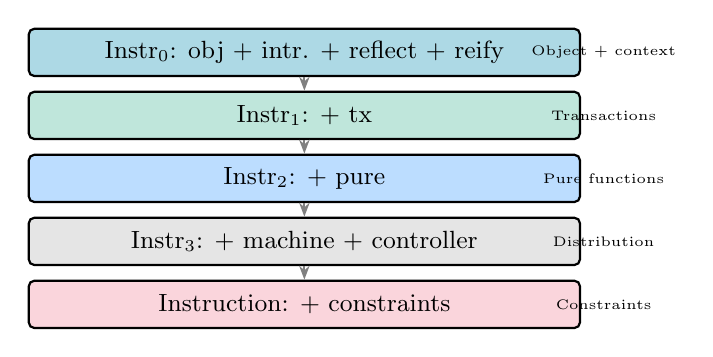
\begin{tikzpicture}[node distance=0.8cm,font=\small]
  % Layer stack (5 layers)
  \node[state,fill=lightblue,minimum width=7cm,minimum height=0.6cm] (l0) {Instr$_0$: obj + intr. + reflect + reify};
  \node[state,fill=junglegreen!30,minimum width=7cm,minimum height=0.6cm,below of=l0] (l1) {Instr$_1$: + tx};
  \node[state,fill=dodgerblue!30,minimum width=7cm,minimum height=0.6cm,below of=l1] (l2) {Instr$_2$: + pure};
  \node[state,fill=gray!20,minimum width=7cm,minimum height=0.6cm,below of=l2] (l3) {Instr$_3$: + machine + controller};
  \node[state,fill=nicered!20,minimum width=7cm,minimum height=0.6cm,below of=l3] (l4) {Instruction: + constraints};

  % Inclusion arrows
  \draw[edge,draw=gray] (l0) -- (l1);
  \draw[edge,draw=gray] (l1) -- (l2);
  \draw[edge,draw=gray] (l2) -- (l3);
  \draw[edge,draw=gray] (l3) -- (l4);

  % Side annotations
  \node[right of=l0,xshift=3cm,font=\tiny,align=left] {Object + context};
  \node[right of=l1,xshift=3cm,font=\tiny,align=left] {Transactions};
  \node[right of=l2,xshift=3cm,font=\tiny,align=left] {Pure functions};
  \node[right of=l3,xshift=3cm,font=\tiny,align=left] {Distribution};
  \node[right of=l4,xshift=3cm,font=\tiny,align=left] {Constraints};
\end{tikzpicture}

\column{0.52\textwidth}
\centering

\textbf{Programs are ITrees}\\

\begin{lstlisting}[basicstyle=\ttfamily\scriptsize]
AVMProgram : Set → Set
AVMProgram = ITree (Instruction Safe)
\end{lstlisting}

\vspace{0.4em}

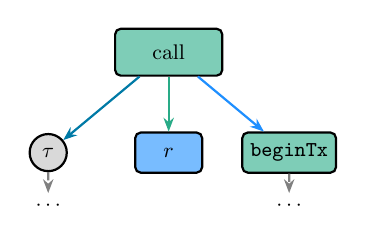
\begin{tikzpicture}[x=1cm,y=1cm,font=\small,scale=0.85,transform shape]
  % Root event
  \node[event,minimum width=1.6cm,minimum height=0.7cm] (call) at (0,0) {\lstinline{call}};

  % Branch targets
  \node[silent,minimum size=5mm] (tau1) at (-1.8,-1.5) {$\tau$};
  \node[result,minimum width=1cm,minimum height=0.6cm] (ret)  at (0,-1.5) {$r$};
  \node[event,minimum width=1.4cm,minimum height=0.6cm]  (write) at (1.8,-1.5) {\texttt{beginTx}};

  % Continuations
  \node at (-1.8,-2.3) (cont1) {$\cdots$};
  \node at (1.8,-2.3)  (cont2) {$\cdots$};

  % Edges
  \draw[edge,thick] (call) -- node[above left,font=\tiny] {} (tau1);
  \draw[resp,thick] (call) -- node[right,font=\tiny] {} (ret);
  \draw[msg,thick]  (call) -- node[above right,font=\tiny] {} (write);
  \draw[edge,draw=gray,dashed] (tau1) -- (cont1);
  \draw[edge,draw=gray,dashed] (write) -- (cont2);
\end{tikzpicture}

{\scriptsize Tree branches = possible return values (e.g., \lstinline{call} returns \lstinline{Maybe Output})}

\end{columns}

\vspace{0.6em}

\textbf{Design principle:} Layered inclusion (not horizontal composition)

{\small
\[
  \text{Instr}_0 \subseteq \text{Instr}_1 \subseteq \text{Instr}_2 \subseteq \text{Instr}_3 \subseteq \text{Instruction}
\]}

\end{frame}

%------------------------------------------------

\begin{frame}[fragile]{How do we separate ``where'' from ``who''?}

\begin{columns}[T]
\column{0.48\textwidth}

\textbf{Machines} (Physical layer)
\begin{itemize}\small
  \item Physical compute nodes (servers)
  \item Store (local) object data and run programs
  \item Objects have a \lstinline{machine} field in metadata
  \item \lstinline{teleport}: Move \textit{execution context} to another machine
  \item \lstinline{moveObject}: Move the actual* object to another machine
\end{itemize}

\vspace{0.8em}

\textbf{Controllers} (Logical layer)
\begin{itemize}\small
  \item Logical authority domains
  \item Order transactions for owned objects
  \item Object metadata has \lstinline{currentController}
  \item \lstinline{transferObject}: Change ownership, and more ...
  % \item \texttt{freeze}: Synchronize replicas
\end{itemize}

\column{0.52\textwidth}
\vfill
\vspace{0.5em}

\begin{center}
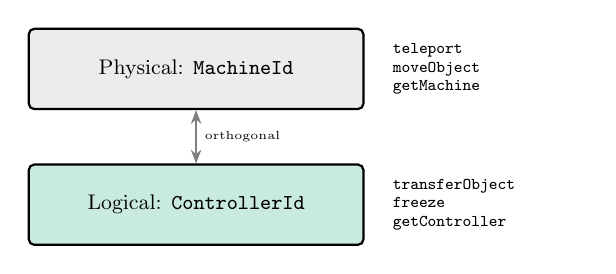
\begin{tikzpicture}[node distance=1cm,font=\small,scale=0.85,transform shape]
  % Layered boxes
  \node[state,fill=gray!15,minimum width=5cm,minimum height=1.2cm] (phys) {Physical: \texttt{MachineId}};
  \node[state,fill=junglegreen!25,minimum width=5cm,minimum height=1.2cm,below=0.8cm of phys] (logic) {Logical: \texttt{ControllerId}};

  % Annotations
  \node[right=0.3cm of phys,font=\scriptsize,text width=2.8cm,align=left] {
    \texttt{teleport}\\
    \texttt{moveObject}\\
    \texttt{getMachine}
  };
  \node[right=0.3cm of logic,font=\scriptsize,text width=2.8cm,align=left] {
    \texttt{transferObject}\\
    \texttt{freeze}\\
    \texttt{getController}
  };

  % Relationship
  \draw[edge,draw=gray,<->] (phys) -- node[right,font=\tiny,black] {orthogonal} (logic);
\end{tikzpicture}
\end{center}

\vspace{0.5em}

{\footnotesize\textbf{Key insight:} Physical location (where data lives) is independent of logical authority (who controls it)}
\vfill

\end{columns}

\end{frame}

%------------------------------------------------

%----------------------------------------------------------------------------------------
%    PART IV: INSTRUCTION LAYERS (OVERVIEW)
%----------------------------------------------------------------------------------------

\section{Instruction Layers}

\begin{frame}{What can objects do? (Instr$_0$)}

\vfill

\begin{columns}[T]
\column{0.48\textwidth}

\textbf{Object lifecycle and communication}

\begin{itemize}\small
  \item \texttt{createObj}: Create new object
  \item \texttt{destroyObj}: Destroy object
  \item \texttt{call}: Send message to object
  \item \texttt{receive}: Receive incoming message
\end{itemize}

\vspace{0.5em}

\textbf{Introspection} {\small (self-examination, safe)}

\begin{itemize}\small
  \item \texttt{self}: Get current object ID
  \item \texttt{input}: Get current input
  \item \texttt{history}: Get input sequence
  \item \texttt{sender}: Get sender object ID
\end{itemize}

\column{0.48\textwidth}

\textbf{Reflection} {\small (examining others, unsafe)}

\begin{itemize}\small
  \item \texttt{reflect}: Examine object metadata
  \item \texttt{scryMeta}: Query objects by metadata
  \item \texttt{scryDeep}: Query by behavior + metadata
\end{itemize}

\vspace{0.5em}

\textbf{Reification} {\small (capture state as data)}

\begin{itemize}\small
  \item \texttt{reifyContext}: Capture execution context
  \item \texttt{reifyTxState}: Capture transaction state (unsafe)
  \item \texttt{reifyConstraints}: Capture constraint state (unsafe)
\end{itemize}

\end{columns}

\vfill

\end{frame}

%------------------------------------------------

\begin{frame}{How do we get atomicity? (Instr$_1$)}

\vfill

\textbf{Atomic execution contexts}

\begin{itemize}
  \item \texttt{beginTx}: Start new transaction $\to$ \texttt{TxId}
  \item \texttt{commitTx}: Validate and apply changes $\to$ \texttt{Bool} (may fail on conflict)
  \item \texttt{abortTx}: Discard all changes
\end{itemize}

\vspace{1em}

\textbf{Transaction semantics:}

\begin{itemize}
  \item \textbf{\texttt{beginTx}:} Initializes empty overlays (\texttt{txLog}, \texttt{creates}, \texttt{destroys}, \texttt{observed})
  \item \textbf{\texttt{commitTx}:} Validates observed versions, applies all pending changes atomically
  \item \textbf{\texttt{abortTx}:} Discards all pending changes, clears overlays
\end{itemize}

\vspace{0.5em}

\textbf{Conflict detection:} Read set (\texttt{observed}) checked against current store versions

\vfill

\end{frame}

%------------------------------------------------

\begin{frame}{How do objects move across machines? (Instr$_3$)}

\vfill

\begin{columns}[T]
\column{0.48\textwidth}

\textbf{Machine Layer} (Physical)

\vspace{0.3em}

\begin{itemize}\small
  \item \texttt{getMachine}: Get object's machine
  \item \texttt{teleport}: Move execution to another machine
  \item \texttt{moveObject}: Move object data to another machine
  \item \texttt{fetch}: Bring object replica locally
\end{itemize}

\vspace{0.5em}

\textbf{Properties:}
\begin{itemize}\scriptsize
  \item Invalid during active transactions
  \item Affects physical data location
\end{itemize}

\column{0.48\textwidth}

\textbf{Controller Layer} (Logical)

\vspace{0.3em}

\begin{itemize}\small
  \item \texttt{getCurrentController}: Get current controller
  \item \texttt{getController}: Get object's controller
  \item \texttt{transferObject}: Change object ownership
  \item \texttt{freeze}: Synchronize object replicas
\end{itemize}

\vspace{0.5em}

\textbf{Properties:}
\begin{itemize}\scriptsize
  \item Affects logical authority
  \item Transactional ownership transfer
\end{itemize}

\end{columns}

\vfill

\end{frame}

%------------------------------------------------

\begin{frame}{What about pure computation? (Instr$_2$)}

\vfill

\textbf{Pure Function Layer}

\vspace{0.5em}

\begin{columns}[T]
\column{0.48\textwidth}

\textbf{Core instructions:}

\begin{itemize}
  \item \texttt{callPure}: Invoke registered function
  \item \texttt{registerPure}: Add new function (unsafe)
  \item \texttt{updatePure}: Modify existing function (safe)
\end{itemize}

\vspace{0.5em}

{\small All functions are side-effect free: \texttt{List Val → Maybe Val}}

\column{0.48\textwidth}

\textbf{Key properties:}

\begin{itemize}\small
  \item Extensible function registry
  \item Side-effect free computation
  \item No object overhead
  \item \texttt{registerPure} modifies global state (unsafe)
\end{itemize}

\vspace{0.5em}

{\footnotesize Enables reusable logic without creating objects}

\end{columns}

\vfill

\end{frame}

%------------------------------------------------

\begin{frame}{How do we support intent matching?}

\vfill

\centering
\textbf{Constraint Programming Instructions}

\vspace{0.5em}

\begin{columns}[t]
\column{0.32\textwidth}

\textbf{FD Constraints}\\
{\scriptsize (Call-time choice)}

\vspace{0.3em}

\begin{itemize}\scriptsize
  \item \texttt{newVar}: Create FD variable with domain
  \item \texttt{narrow}: Restrict variable domain
  \item \texttt{post}: Add constraint (e.g., $x < y$)
  \item \texttt{label}: Assign concrete value
\end{itemize}

\vspace{0.2em}

{\tiny CSP-style with incremental propagation}

\column{0.32\textwidth}

\textbf{Nondeterminism}\\
{\scriptsize (Commit-time validation)}

\vspace{0.3em}

\begin{itemize}\scriptsize
  \item \texttt{choose}: Select from alternatives non-deterministically
  \item \texttt{require}: Assert boolean constraint must hold
\end{itemize}

\vspace{0.2em}

{\tiny Constraints accumulate during execution, solved externally at commit}

\column{0.32\textwidth}

\textbf{Linear Constraints}\\
{\scriptsize (Resource tracking)}

\vspace{0.3em}

\begin{itemize}\scriptsize
  \item \texttt{newLinearConstraint}: Create resource equation
  \item \texttt{satisfyLinear}: Verify resource balance
\end{itemize}

\vspace{0.2em}

{\tiny Linear resource accounting and verification}

\end{columns}

\vfill

\end{frame}

%------------------------------------------------

%----------------------------------------------------------------------------------------
%    PART V: EXAMPLE
%----------------------------------------------------------------------------------------

\section{Complete Example}

\begin{frame}[fragile]{How does it work in practice?}

\textbf{Example:} Atomic Transfer

\begin{columns}[T]
\column{0.54\textwidth}

\textbf{Scenario:} Transfer tokens between accounts atomically

\vspace{0.5em}

\begin{lstlisting}[basicstyle=\ttfamily\scriptsize]
transfer : ObjectId → ObjectId → ℕ
         → AVMProgram Bool
transfer alice bob amount = do
  txId ← beginTx

  -- Debit Alice's account
  r1 ← call alice (debit amount)

  -- Credit Bob's account
  r2 ← call bob (credit amount)

  -- Commit if both succeed
  case (r1 , r2) of
    (just _ , just _) → commitTx txId
    _                 → abortTx txId
                        >> return false
\end{lstlisting}

\column{0.46\textwidth}

\vspace{2em}

\textbf{Transaction guarantees:}

\vspace{0.5em}

\begin{itemize}\small
  \item \textbf{Atomicity:} Both updates happen or neither does

  \vspace{0.3em}

  \item \textbf{Isolation:} Changes invisible until commit

  \vspace{0.3em}

  \item \textbf{Consistency:} Version checking detects concurrent modifications

  \vspace{0.3em}

  \item \textbf{Conflict handling:} \lstinline{commitTx} returns \lstinline{false} on conflict
\end{itemize}

\vspace{1em}

{\footnotesize\textbf{Execution:} Cannot handle objects from more than one controller within a transaction. However, \lstinline{transferObject} can change ownership during the transaction.}

\end{columns}

\end{frame}

%------------------------------------------------


%----------------------------------------------------------------------------------------
%    PART VI: CONCLUSION
%----------------------------------------------------------------------------------------

\section{Conclusion}

\begin{frame}{Summary}

\vfill

\textbf{The AVM specification defines:}

\vspace{0.5em}

\begin{columns}[T]
\column{0.48\textwidth}
\textbf{Design Principles}

\begin{itemize}
  \item \textbf{Layered ISA} \\
  {\small Five layers of inclusion: Instr$_0$ $\subseteq$ Instr$_1$ $\subseteq$ Instr$_2$ $\subseteq$ Instr$_3$ $\subseteq$ Instruction}

  \item \textbf{Two-level distribution} \\
  {\small Physical (machines) vs Logical (controllers)}

  \item \textbf{Formal semantics} \\
  {\small Interaction trees + machine-checked Agda specification}
\end{itemize}

\column{0.48\textwidth}
\textbf{Instruction Set + Semantics}

\begin{itemize}
  \item \textbf{Objects \& introspection} \\
  {\small Message-driven with reflection and reification}

  \item \textbf{Transactions} \\
  {\small Atomic blocks with serializable snapshot isolation}

  \item \textbf{Constraint programming} \\
  {\small FD constraints, nondeterminism, linear resources}

  \item \textbf{Distribution} \\
  {\small Object migration and ownership transfer}
\end{itemize}
\end{columns}

\vspace{0.5em}

{\footnotesize\textbf{Note:} Provides instructions and expected semantics, not production interpreter implementation}

\vfill

\end{frame}

%------------------------------------------------

% (Removed implementation status slide to avoid future-work/status content)
% (Removed "Explore the Specification" slide)

%----------------------------------------------------------------------------------------
%    BONUS MATERIAL
%----------------------------------------------------------------------------------------

\section*{Bonus Material}

%------------------------------------------------

\begin{frame}{Bonus Slides}

\vfill

\begin{center}
\Large \textbf{Additional Technical Details}
\end{center}

\vspace{1em}

\centering
\begin{itemize}
  \item Core Abstractions (state, messaging, tx semantics)
  \item Instruction Details \& Error Stack
  \item Result Types \& Interpreter Structure
  \item System Model (Assumptions)
  \item Object Ownership Transfer
  \item Pure Instructions \& Safety-Indexed Operations
\end{itemize}

\vfill

\end{frame}

%------------------------------------------------

\subsection*{Core Abstractions (Bonus)}

\begin{frame}{What is an object?}

\textbf{Two components:} Abstract behavior + Runtime metadata

\begin{columns}[T]
\column{0.48\textwidth}
\textbf{Abstract Object} \\
{\small (AVM program / Module parameter)}

\vspace{0.3em}

Module is parameterized by:
\begin{itemize}\scriptsize
  \item \texttt{Val}: Value type
  \item \texttt{ObjectId}: Object identifiers
  \item \texttt{MachineId}: Physical nodes
  \item \texttt{ControllerId}: Logical authorities
  \item \texttt{TxId}: Transaction identifiers
  \item \texttt{ObjectBehaviour}: Program behavior
\end{itemize}

\column{0.48\textwidth}
\textbf{Runtime Metadata} \\
{\small (Managed by AVM)}

\vspace{0.3em}

Each object tracks:
\begin{itemize}\scriptsize
  \item \texttt{objectId}: Unique identifier
  \item \texttt{history}: Message sequence
  \item \texttt{machine}: Physical location (where)
  \item \texttt{creatingController}: Origin authority
  \item \texttt{currentController}: Current authority (who)
\end{itemize}

\vspace{0.5em}

{\scriptsize History grows monotonically—objects compute behavior by replaying full message sequence}

\end{columns}

\vspace{0.5em}

\textbf{Separation:} Objects (AVM programs, immutable) vs. Metadata (mutable runtime state)

\end{frame}

%------------------------------------------------

\begin{frame}{What does the runtime track?}

\begin{columns}[T]
\column{0.52\textwidth}

\textbf{Five logical components:}

\begin{enumerate}\scriptsize
  \item \textbf{Physical context}\\
  \texttt{machineId}: Current machine

  \item \textbf{Controller context}\\
  \texttt{controllerId}: Current authority

  \item \textbf{Persistent storage}\\
  \texttt{store}: Objects + metadata maps

  \item \textbf{Transactional overlay}\\
  \texttt{txLog}, \texttt{creates}, \texttt{destroys}, \texttt{observed}, \texttt{pendingTransfers}

  \item \textbf{Execution frame}\\
  \texttt{self}, \texttt{input}, \texttt{sender}, \texttt{traceMode}
\end{enumerate}

\column{0.48\textwidth}

\textbf{Store separation:}

\vspace{0.3em}

\begin{itemize}\scriptsize
  \item \texttt{objects}: ObjectId $\to$ Maybe Object
  \item \texttt{metadata}: ObjectId $\to$ Maybe ObjectMeta
\end{itemize}

\vspace{0.5em}

\textbf{Key design:}

\begin{itemize}\scriptsize
  \item \textbf{Physical context:} Machine identity
  \item \textbf{Controller context:} Logical authority
  \item \textbf{Persistent storage:} Objects + metadata
  \item \textbf{Transactional overlay:} Pending changes
  \item \textbf{Execution frame:} Current call context + trace
\end{itemize}

\end{columns}

\end{frame}

%------------------------------------------------

\begin{frame}{How do objects communicate?}

\begin{columns}[T]
\column{0.45\textwidth}

\textbf{The only way to interact with objects:}

\vspace{0.3em}

\texttt{call}: ObjectId $\to$ Input $\to$ Maybe Output

\vspace{0.5em}

\textbf{Behavior from full history:}

\vspace{0.3em}

Object behavior = \texttt{getBehavior(history ++ [newInput])}

\vspace{0.5em}

\textbf{Key properties:}

\begin{itemize}\scriptsize
  \item \textbf{No hidden state:} History is the state
  \item \textbf{Transactional:} Pending inputs until commit
  \item \textbf{Replay semantics:} Full recomputation on each call
\end{itemize}

\column{0.55\textwidth}

\begin{center}
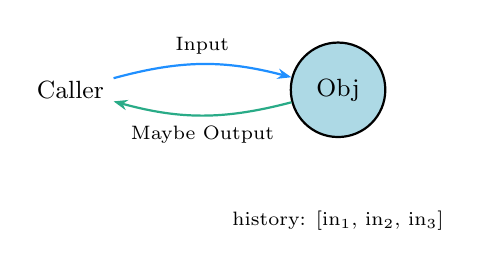
\begin{tikzpicture}[node distance=1.2cm,font=\small]
  \node[object,minimum size=12mm] (obj) {Obj};
  \node[left of=obj,xshift=-2.2cm] (caller) {Caller};

  \draw[msg] (caller) to[bend left=15] node[above,font=\scriptsize] {Input} (obj);
  \draw[resp] (obj) to[bend left=15] node[below,font=\scriptsize] {Maybe Output} (caller);

  \node[below=0.8cm of obj,font=\scriptsize] {
    history: [in$_1$, in$_2$, in$_3$]
  };
\end{tikzpicture}
\end{center}

\vspace{1em}

{\small Each \texttt{call} appends to history; behavior is recomputed from scratch on the full sequence}

\end{columns}

\end{frame}

%------------------------------------------------

\begin{frame}{How do transactions work?}

\begin{columns}[T]
\column{0.45\textwidth}

\textbf{Transactions within a controller}

\vspace{0.2em}

{\small True atomicity requires single-controller scope}

\vspace{0.3em}

\textbf{Three instructions:}

\begin{itemize}\scriptsize
  \item \texttt{beginTx} — Start atomic block (returns TxId)
  \item \texttt{commitTx} — Persist all changes (may fail on conflict)
  \item \texttt{abortTx} — Discard all changes (always succeeds)
\end{itemize}

\vspace{0.3em}

{\scriptsize\textbf{Controller-locality:} \texttt{call}, \texttt{destroyObj}, \texttt{transferObject} target only owned objects}

\column{0.55\textwidth}

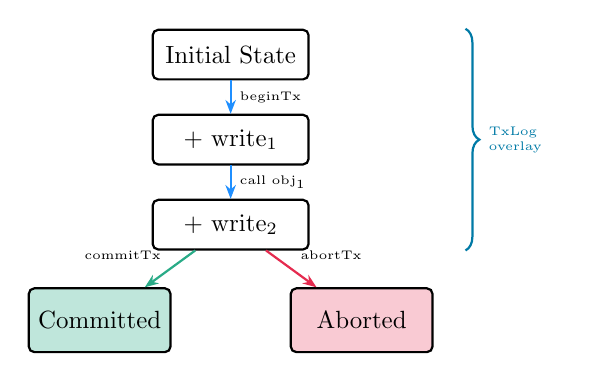
\begin{tikzpicture}[node distance=1.2cm,scale=0.9,transform shape]
  % States
  \node[state,minimum width=2.2cm,minimum height=0.7cm] (s0) {Initial State};
  \node[state,below of=s0,minimum width=2.2cm,minimum height=0.7cm] (s1) {+ write$_1$};
  \node[state,below of=s1,minimum width=2.2cm,minimum height=0.7cm] (s2) {+ write$_2$};
  \node[final,below left of=s2,xshift=-1cm,yshift=-0.5cm,minimum width=2cm] (commit) {Committed};
  \node[abort,below right of=s2,xshift=1cm,yshift=-0.5cm,minimum width=2cm] (abort) {Aborted};

  % Arrows
  \draw[msg] (s0) -- node[right,black,font=\tiny] {beginTx} (s1);
  \draw[msg] (s1) -- node[right,black,font=\tiny] {call obj$_1$} (s2);
  \draw[resp] (s2) -- node[above left,black,font=\tiny] {commitTx} (commit);
  \draw[edge,draw=nicered] (s2) -- node[above right,black,font=\tiny] {abortTx} (abort);

  % Overlay annotation bracket (opening to the left)
  \draw[decorate,decoration={brace,amplitude=5pt},thick,darkblue]
    ([xshift=2.2cm]s0.north east) -- ([xshift=2.2cm]s2.south east)
    node[midway,right,xshift=0.2cm,text width=1.1cm,align=left,font=\tiny] {TxLog\\overlay};
\end{tikzpicture}

\end{columns}

\end{frame}

%------------------------------------------------

\subsection*{Instruction Details (Bonus)}


\begin{frame}{Runtime vs VM vs OS Basics}

\vfill

\begin{itemize}
  \item \textbf{Runtime system:} Library + services that let programs run; wraps what the VM needs (support code, services) and can grow into a full programming environment.
  \item \textbf{Virtual machine:} Software abstraction of a machine defining an application's runtime environment; \(\mathsf{VM} = \text{abstract execution model} + \text{bytecode ISA} + \text{formal operational semantics}\).
  \item \textbf{OS vs user-space VM:} OS is a VM for hardware (processes, threads, files) and exports syscalls; user-space VMs expose their own API (IPC, objects, storage) atop the OS.
  \item \textbf{Notes:} Address space bounds what threads in a process can access; user-space VMs have a long history (e.g., Smalltalk compiler + interpreter).
\end{itemize}

\vfill

\end{frame}

%------------------------------------------------

\begin{frame}{How do we support pure computation? (Instr$_2$)}

\vfill

\begin{columns}[T]
\column{0.52\textwidth}
\textbf{Pure Function Layer}

\vspace{0.5em}

\begin{itemize}
  \item \texttt{callPure}: Invoke registered function
  \item \texttt{registerPure}: Add new function (unsafe)
  \item \texttt{updatePure}: Modify existing function (safe)
\end{itemize}

\vspace{0.5em}

{\small All functions are side-effect free: \texttt{List Val → Maybe Val}}

\column{0.44\textwidth}

\textbf{Design rationale:}

\begin{itemize}\small
  \item Extensible function registry
  \item Side-effect free computation
  \item \texttt{registerPure} is unsafe (modifies global state)
  \item \texttt{updatePure} is safe (requires prior registration)
\end{itemize}

\vspace{0.5em}

{\scriptsize Pure functions enable reusable logic without object overhead}

\end{columns}

\vfill

\end{frame}

%------------------------------------------------

\begin{frame}{How do errors propagate through layers?}

\vfill

\centering
\textbf{Error types match instruction layers:}

\vspace{0.5em}

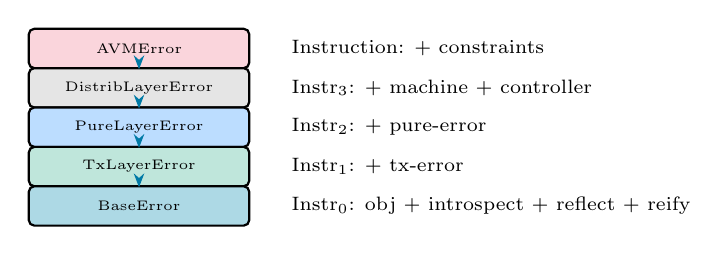
\begin{tikzpicture}[node distance=0.5cm,font=\tiny,
  errbox/.style={rectangle,draw,thick,rounded corners=2pt,minimum width=2.8cm,minimum height=0.5cm}]

  \node[errbox,fill=nicered!20] (avm) {AVMError};
  \node[errbox,fill=gray!20,below of=avm] (distrib) {DistribLayerError};
  \node[errbox,fill=dodgerblue!30,below of=distrib] (pure) {PureLayerError};
  \node[errbox,fill=junglegreen!30,below of=pure] (tx) {TxLayerError};
  \node[errbox,fill=lightblue,below of=tx] (base) {BaseError};

  \draw[edge] (distrib) -- (avm);
  \draw[edge] (pure) -- (distrib);
  \draw[edge] (tx) -- (pure);
  \draw[edge] (base) -- (tx);

  \node[right=0.4cm of avm,font=\scriptsize,align=left] {Instruction: + constraints};
  \node[right=0.4cm of distrib,font=\scriptsize,align=left] {Instr$_3$: + machine + controller};
  \node[right=0.4cm of pure,font=\scriptsize,align=left] {Instr$_2$: + pure-error};
  \node[right=0.4cm of tx,font=\scriptsize,align=left] {Instr$_1$: + tx-error};
  \node[right=0.4cm of base,font=\scriptsize,align=left] {Instr$_0$: obj + introspect + reflect + reify};
\end{tikzpicture}

\vspace{0.5em}

{\small\textbf{Key:} Each layer wraps errors from lower layers plus its own specific errors}

\vfill

\end{frame}

%------------------------------------------------

\subsection*{Execution Details (Bonus)}

\begin{frame}{What do instructions return?}

\begin{columns}[T]
\column{0.52\textwidth}

\textbf{Instruction execution returns:}

\vspace{0.3em}

Success contains:
\begin{itemize}\scriptsize
  \item \texttt{value}: Return value
  \item \texttt{state}: Updated state
  \item \texttt{trace}: Execution trace
\end{itemize}

\vspace{0.3em}

Result is either:
\begin{itemize}\scriptsize
  \item \texttt{success}: Success value
  \item \texttt{failure}: Error value
\end{itemize}

\column{0.48\textwidth}

\textbf{Layer-specific result types:}

\vspace{0.3em}

\begin{itemize}\scriptsize
  \item \texttt{BaseResult A} = Result A BaseError
  \item \texttt{TxResult A} = Result A TxLayerError
  \item \texttt{PureResult A} = Result A PureLayerError
  \item \texttt{AVMResult A} = Result A AVMError
\end{itemize}

\vspace{0.5em}

{\small Each layer refines error types while preserving success structure}

\end{columns}

\end{frame}

%------------------------------------------------

\begin{frame}{How are programs executed?}

\vfill

\textbf{Each instruction family has an interpreter:}

\vspace{0.3em}

\begin{itemize}\scriptsize
  \item \texttt{executeObj}: Object operations
  \item \texttt{executeIntrospect}: Self-examination
  \item \texttt{executeReflect}: Examine others
  \item \texttt{executeReify}: Capture state as data
  \item \texttt{executeTx}: Transactions
  \item \texttt{executePure}: Pure functions
\end{itemize}

\vspace{0.5em}

\textbf{Layered interpreters dispatch by pattern matching:}

\vspace{0.3em}

Each layer executor dispatches to appropriate instruction family executor, building up from Instr$_0$ $\to$ Instr$_1$ $\to$ $\cdots$ $\to$ Instruction

\vspace{0.5em}

\textbf{Program interpreters recursively process ITrees:}

\vspace{0.3em}

\centering
\texttt{interpretAVMProgram}: AVMProgram A $\to$ State $\to$ AVMResult A

\vfill

\end{frame}

%------------------------------------------------

\begin{frame}{What can we assume? What do we guarantee?}

\begin{columns}[T]
\column{0.48\textwidth}

\textbf{Assumptions (Environment)}
\begin{itemize}\small
  \item \textbf{Network:} Asynchronous, reliable, FIFO per sender-receiver
  \item \textbf{Failures:} Crash-stop nodes (no Byzantine faults)
  \item \textbf{Time:} No global clock
\end{itemize}

\column{0.48\textwidth}

\textbf{Guarantees (AVM Model)}
\begin{itemize}\small
  \item \textbf{Atomicity:} Instructions are all-or-nothing; no partial visibility
  \item \textbf{Isolation:} Per-controller Serializable Snapshot Isolation (SSI)
  \item \textbf{Authority:} Invariant: exactly one \texttt{currentController} per object
\end{itemize}

\end{columns}

\vspace{0.8em}

{\footnotesize See \texttt{AVM/SystemModel.md} for complete specification of assumptions}

\end{frame}

%------------------------------------------------

\begin{frame}{How do we transfer ownership?}

\begin{columns}[T]
\column{0.48\textwidth}

\textbf{transferObject Semantics}

\vspace{0.3em}

\texttt{transferObject}: ObjectId $\to$ ControllerId $\to$ Bool

\vspace{0.5em}

\textbf{Execution steps:}
\begin{enumerate}\small
  \item Validate current controller has authority
  \item Update \texttt{currentController} in metadata
  \item Record in pending transfers (if in tx)
  \item Return success/failure
\end{enumerate}

\column{0.48\textwidth}

\textbf{Key properties:}

\begin{itemize}\small
  \item \textbf{Atomic:} Single instruction
  \item \textbf{Authorized:} Only current controller can transfer
  \item \textbf{Transactional:} Respects tx boundaries
\end{itemize}

\vspace{0.5em}

\textbf{ObjectMeta changes:}

\vspace{0.3em}

Before: \texttt{currentController = controllerA}

After: \texttt{currentController = controllerB}

\end{columns}

\vspace{0.5em}

{\footnotesize\textbf{Note:} This is a logical authority change, not a physical move (use \texttt{moveObject} for that)}

\end{frame}

%------------------------------------------------

\begin{frame}{How do we support pure computation? (Instr$_2$)}

\begin{columns}[T]
\column{0.52\textwidth}
\textbf{Pure Function Layer}

\vspace{0.5em}

\begin{itemize}
  \item \texttt{callPure}: Invoke registered function
  \item \texttt{registerPure}: Add new function (unsafe)
  \item \texttt{updatePure}: Modify existing function (safe)
\end{itemize}

\vspace{0.5em}

{\small All functions are side-effect free: \texttt{List Val → Maybe Val}}

\column{0.44\textwidth}

\textbf{Design rationale:}

\begin{itemize}\small
  \item Extensible function registry
  \item Side-effect free computation
  \item \texttt{registerPure} is unsafe (modifies global state)
  \item \texttt{updatePure} is safe (requires prior registration)
\end{itemize}

\vspace{0.5em}

{\scriptsize Pure functions enable reusable logic without object overhead}

\end{columns}

\end{frame}

%------------------------------------------------

\begin{frame}{What makes an operation safe or unsafe?}

\begin{columns}[T]
\column{0.48\textwidth}
\textcolor{dodgerblue}{\textbf{Safe}}
\begin{itemize}
  \item Respects encapsulation
  \item Bounded computation
  \item Message-passing only
  \item Examples: \texttt{call}, \texttt{self}, \texttt{reifyContext}
\end{itemize}

\column{0.48\textwidth}
\textcolor{nicered}{\textbf{Unsafe}}
\begin{itemize}
  \item Breaks encapsulation
  \item Unbounded computation
  \item Direct metadata/object access
  \item Examples: \texttt{scryDeep}, \texttt{reflect}, \texttt{reifyTxState}
\end{itemize}
\end{columns}

\vspace{1em}

\textbf{Three related concepts:}
\begin{itemize}
  \item \textbf{Introspection:} Self-examination (safe) — \texttt{self}, \texttt{history}
  \item \textbf{Reflection:} Examining others (unsafe) — \texttt{reflect}, \texttt{scryDeep}
  \item \textbf{Reification:} Capturing state as data — \texttt{reifyContext}, \texttt{reifyTxState}
\end{itemize}

\end{frame}

%------------------------------------------------

% \begin{frame}{References}
% \bibliography{../specs/references/ref}
% \end{frame}

\end{document}
